\chapter{Optimizations}

If certain characteristics of the UDF are detected optimized translation templates which exploit those characteristics can be chosen. This may either improve performance or enables us to implement work-arounds for settings where the original templates are not applicable otherwise.

To make these optimizations no change in the scenario analysis is required. Instead the scenarios of the UDF are tested for the properties and the results are included in the intermediate representation. so that This enables the best template to be chosen.

\section{Single Recursion}

\begin{wrapfigure}{r}{0.2\textwidth}
  \vspace{-10pt}
  \centering
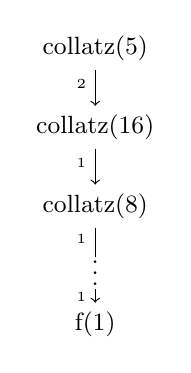
\begin{tikzpicture}\small
% nodes
\node (f1) at (0, 2) {collatz(5)};
\node (f2) at (0, 1) {collatz(16)};
\node (f3) at (0, 0) {collatz(8)};
\node (fn) at (0, -0.75) {$\vdots$};
\node (f0) at (0, -1.5) {f(1)};
% arrows
\draw[->] (f1) --node[pos=0.4, left, label distance=5mm]{\tiny{2}} (f2);
\draw[->] (f2) --node[pos=0.4, left, label distance=5mm]{\tiny{1}} (f3);
\draw (f3) --node[pos=0.4, left, label distance=5mm]{\tiny{1}} +(0, -0.65);
\draw[<-] (f0) --node[pos=0.4, left, label distance=5mm]{\tiny{1}} +(0, 0.45);
\end{tikzpicture}
  \vspace{-10pt}
  \caption{Callgraph of \texttt{collatz(5)}}
  \label{tr_callgraph}
\end{wrapfigure}

Single recursive functions are a subgroup of general recursive functions. They have a linear branching behaviour (\autoref{tr_callgraph}). The function as a whole may contain multiple callsites as long as each evaluation scenario contains only a single callsite. This is also the only criterion to detect single recursive functions.

The function that computed the length of the \textit{collatz-series} (\autoref{lst:collatz_udf}) is an example for a single recursive function.

\begin{figure}[h]
    \centering
    \begin{minipage}[b]{.45\linewidth}
    \centering
    \sqlcode{snippets/collatz.sql}
    \subcaption{UDF computing the length of the \textit{collatz-series} for a start number $\texttt{n} > 0$.}
    \label{lst:collatz_udf}
    \end{minipage}
    \begin{minipage}[b]{.5\linewidth}
    \centering\scriptsize
        \begin{tabular}{|p{1em}|p{3.3cm}|p{2.9cm}|}\hline
        \cellcolor{gray!25} & \texttt{\phantom{NOT }n=1} & \texttt{1}\\\hline
        \end{tabular}
        
        \begin{tabular}{|p{1em}|p{3.3cm}|p{2.9cm}|}\hline
        \cellcolor{gray!25} $\ast$ & \texttt{NOT n=1 AND \phantom{NOT }n \% 2 = 0} & \texttt{1 + collatz(n / 2)}\\\hline
        \end{tabular}
        
        \begin{tabular}{|p{1em}|p{3.3cm}|p{2.9cm}|}\hline
        \cellcolor{gray!25} $\ast$ & \texttt{NOT n=1 AND NOT n \% 2 = 0} & \texttt{1 + collatz(3 * n + 1)}\\\hline
        \end{tabular}
        \vspace{2em}
    \subcaption{Scenarios of \texttt{collatz}. Each recursive scenario contains just a single callsite.}\label{collatz_scenarios}
    \end{minipage}
    \caption{}
    \label{collatz_sql_with_scenarios}
\end{figure}

The evaluation thus happens in a strict linear manner. As each scenario depends only on the result of the previous result the work-around (see \autoref{macro:evaluation_cte}) to access all previous computed results becomes unnecessary. In each iteration exactly one result is computed and in the next iteration the dependant scenario will be evaluated. There is no need to add all previous results to the current result in order to have those rows available later (\autoref{opt_sr_evaluation_cte}). Only actually new rows are added to the results.

\begin{figure}[h!]
    \centering
    \begin{minted}{postgresql}
WITH RECRUSIVE
    ...
    evaluation(in_1, res) AS (
        (TABLE basecases)
        
        UNION ( -- was UNION ALL
            WITH e AS (TABLE evaluation)
            (<eval_recursive_scenario_sr(scenario[1])>)
               UNION ALL
            (<eval_recursive_scenario_sr(scenario[2])>)
        )
    )
SELECT ...
    \end{minted}
    \caption{Simplified evaluation-template for single recursive UDFs.}
    \label{opt_sr_evaluation_cte}
\end{figure}

Furthermore, the rather complicated relational division, transposing and filtering for evaluable scenarios (\autoref{macro:recursive_scenario_evaluation}) can be replaced by a much simpler query (\autoref{opt_sr_eval_scenario}). Because each scenario has only a single callsite no grouping/partitioning is required to collect results of dependant callsites and to check whether all dependencies are available. If a result of the callsite is present the scenario can be evaluated. What remains is basically a simple join (\autoref{opt_sr}).

\begin{figure}[h!]
    \centering
    \sqlcode{snippets/opt_sr.sql}
    \caption{Simplified template for single recursive UDFs. Note how the \texttt{FROM}-clause is just a simple join and no \texttt{WHERE} is required anymore.}
    \label{opt_sr_eval_scenario}
\end{figure}



\section{Tail Recursion}

\begin{wrapfigure}{r}{0.5\textwidth}
  \vspace{-10pt}
    \sqlcode{snippets/collatz_tr.sql}
  \caption{Tail recursive formulation of \texttt{collatz}}
  \label{lst:fib_tr}
\end{wrapfigure}

A special form of single recursive functions are tail recursive functions. They do not have any evaluation context around any callsite. Therefore, each recursive scenario just returns another recursive call. Eventually, the result of the basecase is just passed all the way up in the callgraph to the root without any modifications. Hence, this last phase can be skipped, meaning no \texttt{evaluation}-CTE is required.

The final result is present in the \texttt{basecase}-CTE. The basecase-CTE contains only a single value because single recursive functions have no branches in the callgraph (cp. \autoref{tr_callgraph}). The modifications on the template amount to removing the \texttt{evaluation}-CTE and changing result selection as shown in \autoref{tr_opt_template}. Furthermore, the \texttt{callsite\_id}-column can be removed from the \texttt{callgraph}-CTE because the only use of the \texttt{callsite\_id} is to identify the corresponding scenario during evaluation, which now is omitted (\autoref{marco:collect_call_maybe_optimized}).

\begin{figure}
    \centering
    \sqlcode{snippets/opt_tr.sql}
    \caption{Template for tail recursive UDFs. No \texttt{evaluation}-CTE is required anymore as all the basecases already return the final result.}
    \label{tr_opt_template}
\end{figure}


\begin{figure}[h!]\centering\small
    \begin{minted}{postgresql}
    <collect_call_maybe_tr(in_arg_1, predicate, callsite)>
        := SELECT
             in_arg_1                    AS in_1, 
           --callsite.id                 AS callsite_id,
             callsite.arg_1[in_arg_1/$1] AS out_1
           FROM predicate AS p(is_true)
           WHERE p.is_true
    \end{minted}
  \caption{Pseudocode to generate a single call to the callstack-table, optimized for tail recursive UDFs. The callsite id is no longer required as the evaluation-phase is skipped.}
  \label{marco:collect_call_maybe_optimized}
\end{figure}

To test whether an UDF is tail recursive all its scenarios must be tail recursive. This means that the context of the only callsite \texttt{f(...} must be present at the top level of the query or nested in trivial \texttt{SELECT}s. Any computations like \texttt{1+(SELECT f(n))} would create a computation context around the call needing to be evaluated.

\begin{figure}
    \centering
\begin{minted}{postgresql}
q := f(...)
q := (SELECT <q>)
q := (WITH [<alias> AS (<nonrecursive sql>), ...] <q>)
\end{minted}
    \caption{Grammar for tail-recursive queries. This notion could be extended, but catches most cases as it is.}
    \label{tr_grammar}
\end{figure}

CTEs can be included in the query if they are only referenced from the callsite-arguments. Callsite-arguments are evaluated during callgraph creation. During evaluation the callsites including their arguments are replaced by references to their results. Because of this, CTEs are present but unused during evaluation. Therefore the resulting query is eligible for the tail recursive optimization.

\section{Constant argument removal}

Some functions have arguments always just passed on to subsequent calls without modification, eg. configuration parameters. As these parameters do not change it is not necessary to include them in the callgraph-table or when matching rows by arguments. The argument can just be left as it is in the translation, eg. as \texttt{\$1}.

\begin{wrapfigure}{r}{0.66\textwidth}
  \vspace{-10pt}
    \sqlcode{snippets/sieve.sql}
  \caption{Sieve of Eratosthenes. \texttt{sieve(2, ARRAY[1, 2, 3, ..., n])} computes all prime numbers up to \texttt{n}.}
  \label{lst:sieve_udf}
\end{wrapfigure}

Omitting unnecessary arguments saves memory as well as CPU-time. The two tables \texttt{callgraph} and \texttt{evaluation} are joined in each iteration of the \texttt{evaluation}-CTE by the function arguments. Removing unnecessary comparisons speeds up the query and saves memory as the same value is not copied again and again.

No change to the template is necessary and detection of constant arguments is straight-forward: The nth argument of a UDF is constant if the nth argument in each callsite is just \texttt{\$n}. The argument is just removed from the list of arguments thus the argument is not considered when filling out templates.

\begin{figure}[h]
    \centering\footnotesize
    \begin{minipage}[b]{\linewidth}
    \centering
    \begin{tabular}{c|c|c|c|c}
         in\_1 & in\_2                                     & callsite\_id & out\_1 & out\_2                                  \\\hline
         2     & \mintinline{postgresql}{ARRAY[2, 3, ..., 7]} & 1            & 3      & \mintinline{postgresql}{ARRAY[2, 3, ..., 7]}\\
         3     & \mintinline{postgresql}{ARRAY[2, 3, ..., 7]} & 1            & 4      & \mintinline{postgresql}{ARRAY[2, 3, ..., 7]}\\
    \end{tabular}
    \subcaption{\texttt{callgraph}-CTE for \texttt{sieve} without optimization}
    \label{}
    \end{minipage}\par
    \vspace*{15mm}
    \begin{minipage}[b]{\linewidth}
    \centering
    \begin{tabular}{c|c|c}
         in\_1 & in\_2                                     & result                                  \\\hline
         4     & \mintinline{postgresql}{ARRAY[2, 3, ..., 7]} & \mintinline{postgresql}{ARRAY[2, 3, 4, 5, 6, 7]}\\
         3     & \mintinline{postgresql}{ARRAY[2, 3, ..., 7]} & \mintinline{postgresql}{ARRAY[2, 3, 4, 5, 7]}\\
         2     & \mintinline{postgresql}{ARRAY[2, 3, ..., 7]} & \mintinline{postgresql}{ARRAY[2, 3, 5, 7]}\\
    \end{tabular}
    \subcaption{\texttt{evaluation}-CTE for \texttt{sieve} without optimization}
    \label{}
    \end{minipage}
    \caption{}
    \label{}
\end{figure}

\begin{figure}[h]
    \centering
    \begin{minted}{postgresql}
SELECT c.in_1                                  AS in_1, 
       (SELECT array_agg(T.v)
        FROM unnest($2) AS T(v)
        WHERE (T.v = c.in_1 OR T.v % c.in_1 <> 0)
          AND T.v = ANY((SELECT e.result)))       AS result
FROM calls_to_basecases c
WHERE (SELECT (2 * c.out_1) > (array_length($2, 1))
    \end{minted}
    \caption{Evaluation of a nonrecursive scenario of \texttt{sieve} inside the \texttt{basecases}-CTE with constant argument removal. Note that \texttt{\$2} is not replaced by \texttt{c.in\_2}.}
    \label{fig:my_label}
\end{figure}

\section{Handling unhashable types}

In some places within the templates we use the duplicate eliminating \texttt{UNION} which internally depends on the "equals" member of its B-tree operator class \cite[p. 1042 f.]{psql}. Equality can be determined either by sorting, which is used as first choice, or by hashing. Custom types use the sorting operator of its components but lack a default hashing operator.

An undocumented quirk of PostgreSQL is that \texttt{UNION} within \texttt{WITH RECURSIVE} can just use hashing for duplicate elimination\footnote{see \url{https://www.postgresql-archive.org/Hashable-custom-types-td5801576.html}, last accessed at 29/12/2018}. Therefore an error \textit{all column datatype must be hashable} is thrown. This is undesirable because our goal is for the translation to behave exactly like the original and raise no unexpected errors.

A workaround is to cast unhashable types to \texttt{TEXT} when saving in a table and casting it back to the original type whenever using it. Unhashable types can occur in the arguments and in the return type.

If the return type is not hashable the result from each evaluated scenario must be casted to \texttt{TEXT} before storing into \texttt{basecases} or \texttt{evaluation}. When replacing the result of a callsite with a reference to \texttt{evaluation} it must be casted back to the original type. Within the final result selection the result must also be casted back to the original type.

Hashable arguments have to be casted to \texttt{TEXT} when creating the \texttt{callgraph}. To evaluate the callsite-arguments the reference to the \texttt{out}-columns must be casted back to the original type. The same is required when replacing arguments during scenario-evaluation.

Unhashable types are detected by introspecting PostgreSQL (\autoref{sql:hashable_query}). This makes the translation aware of custom hash-operators. PostgreSQL has some type-aliases defined, eg. \texttt{smallint} is an alias for \texttt{int2}. The first is returned by \texttt{t.oid :: regtype} and the latter by \textit{t.typename}.

\begin{figure}
    \centering
\begin{minted}{postgresql}
SELECT t.typname :: TEXT 
FROM pg_operator as o, pg_type as t 
WHERE o.oprleft = t.oid 
  AND o.oprright = t.oid 
  AND o.oprname = '=' 
  AND o.oprcanhash 

UNION

SELECT t.oid :: regtype  :: TEXT 
FROM   pg_operator as o, pg_type as t 
WHERE o.oprleft = t.oid 
  AND o.oprright = t.oid 
  AND o.oprname = '=' 
  AND o.oprcanhash;
\end{minted}
    \caption{Query to obtain all type-aliases from a PostgreSQL-instance that have an operator defined that can be used for hashing.}
    \label{sql:hashable_query}
\end{figure}